\section{Compatibilidad entre Compuertas}

Al momento de adquirir una compuerta lógica comercial, se especifica
en el código el tipo de tecnología que se implementa en dicha compuerta.
Por ejemplo, "HC" hace referencia a "High speed CMOS" mientras
que "HCT" significa "High speed CMOS TTL''   o también existe
"LS'' aludiendo a "Low power schotky". En esta parte del artículo
se analizarán algunas diferencias prácticas entre estos tipos compuertas
y se mencionarán algunos parámetros a tener en cuenta para combinar
más de dos tipos distintos en un mismo circuito.

Para el análisis se utilizarán las siguientes compuertas lógicas:
74HC02, 74HCT02, 74LS02. Estas corresponden a compuertas "NOR".

\subsection{Margen de Ruido}

De la hoja de datos de los distintos componentes se extrajeron los
siguientes parámetros sobre el margen de ruido:

\begin{table}[H]
    \centering
\begin{tabular}{|c|c|c|c|}
\hline 
 & 74HC02 & 74HCT02 & 74LS02\tabularnewline
\hline 
High Level Noise Margin & 1.25V & 2.2V & 0.7V\tabularnewline
\hline 
Low Level Noise Margin & 1.25V & 0.7V & 0.3V\tabularnewline
\hline 
\end{tabular}

\caption{Márgenes de Ruido extraídos de hojas de datos}
\end{table}


\subsection{Conexión entre Compuertas}

Al conexionar entre compuertas, pueden existir problemas al cargar
la tecnología LS con una compuerta de tipo HC. Esto es debido a que
los niveles de entrada (como se puede observar en la tabla expuesta
anteriormente) de la tecnología HC son más restrictivos que los valores
de salida de la LS. Por otro lado, este problema no ocurre cuando
se carga la compuerta LS con una HCT, la cual justamente está pensada
para solucionar los problemas de compatibilidad de una HC.

De todas maneras, aunque el fabricante en la datasheet de su componente
indique valores como los que se han mostrado en el apartado anterior,
en la práctica puede ocurrir que estos parámetros difieran, como por
ejemplo en el caso del margen de ruido. Es decir, que puede ocurrir
que en la practica se pueda interconectar una compuerta LS con una
HC sin tener problemas debido a que el margen de ruido de la LS sea
más elevado de lo que se indica en la hoja de datos. A continuación
se muestra una imagen de una medición realizada con osciloscopio de
la respuesta de una compuerta LS cargada por una HC:

\begin{figure}[H]
\begin{centering}
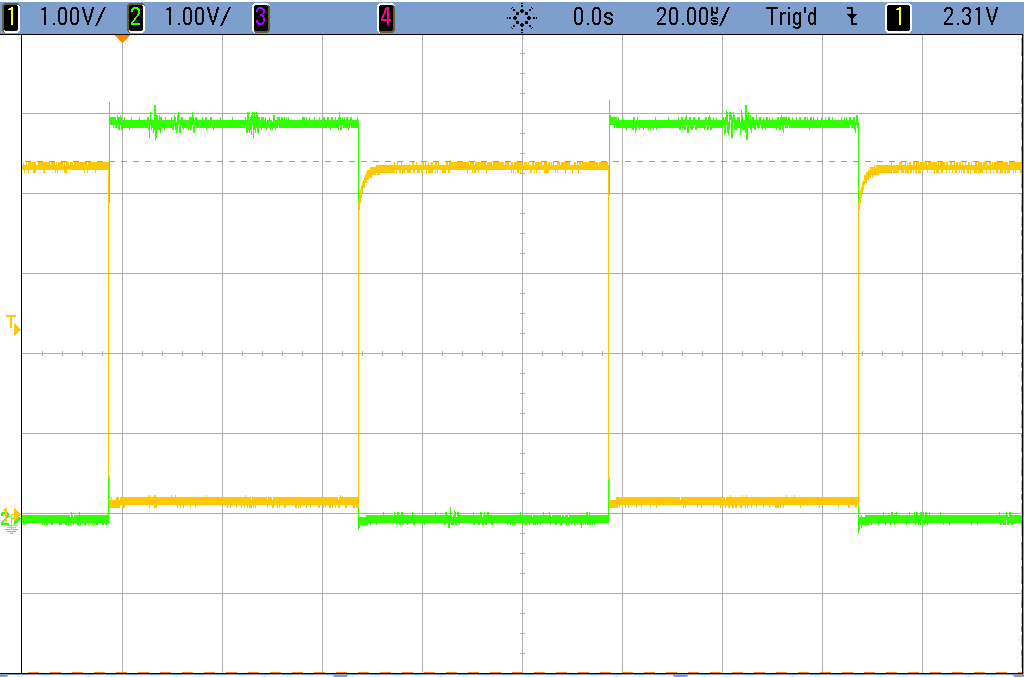
\includegraphics[scale=0.4]{LS-CargadoConHC02}
\par\end{centering}
\caption{Medición - Compuerta LS cargada con HC}
\end{figure}

Las compuertas son NOR que se conexionaron de tal manera que simulan
dos NOT en serie, por ende tiene sentido que cuando una señal está
en alto la otra se mantenga en bajo. Vale aclarar que la señal representada
de color amarillo es la salida de la compuerta HC mientras que la
otra es la correspondiente a la compuerta LS.